\chapter{Optymalizacja}
 
\section{Optymalizacja nastaw regulatora}

Do optymalizacji nastaw regulatorów wykorzystano skrypty zawarte w rozdziale \ref{implementacja}. Badania przeprowadzone zostały dla zestawu parametrów obiektu zaprezentowanego w tabeli \ref{tab_par}. Rząd obiektu jak i wartość zadana były były zmiennymi parametrami i  odpowiednio wartości: \\
$ n \in \{1,2,3\} $ - rząd obiektu, \\
$ z \in \{ 5,10,20,50,70\}$ - wartość zadana \\ 
\subsection{Zestawy parametrów}
W tabeli \ref{tab_par} zamieszczono przyjęte wartości parametrów opisujących obiekt regulacji.
\begin{table}[]
	\centering
	\caption{Zestawy parametrów dla których przeprowadzano optymalizację nastaw regulatorów.}
	\label{tab_par}
	\begin{tabular}{|c|c|} \hline
	Parametr & Wartość \\ \hline
	$K_{w1}$  & 10 \\ \hline
	$K_{w2}$  & 5 \\ \hline
	$T_{w2}$  & 0.1 \\ \hline
	$T_0$   & 1 \\ \hline
	$K_0$   & 10 \\ \hline
	$\tau$ & 1 \\ \hline
	\end{tabular}
\end{table}


\subsection{Optymalizacja nastaw regulatorów}
Dla kolejnych zestawów parametrów opisujących system przeprowadzano procedurę optymalizacji nastaw regulatorów minimalizując wska\'znik jakości opisany zależnością \ref{wsk_jak}. Proces optymalizacji przeprowadzany był dla różnych wartości zadanych w obecności znanego zakłócenia $z_2$ (zakłócenie skokowo zmieniające swoją wartość) oraz nieznanego zakłócenia $z_1$. Przebiegi owych zakłóceń przedstawiono na rysunku \ref{fig_zaklocenia}. 

\begin{figure}[h!]
	\centering
	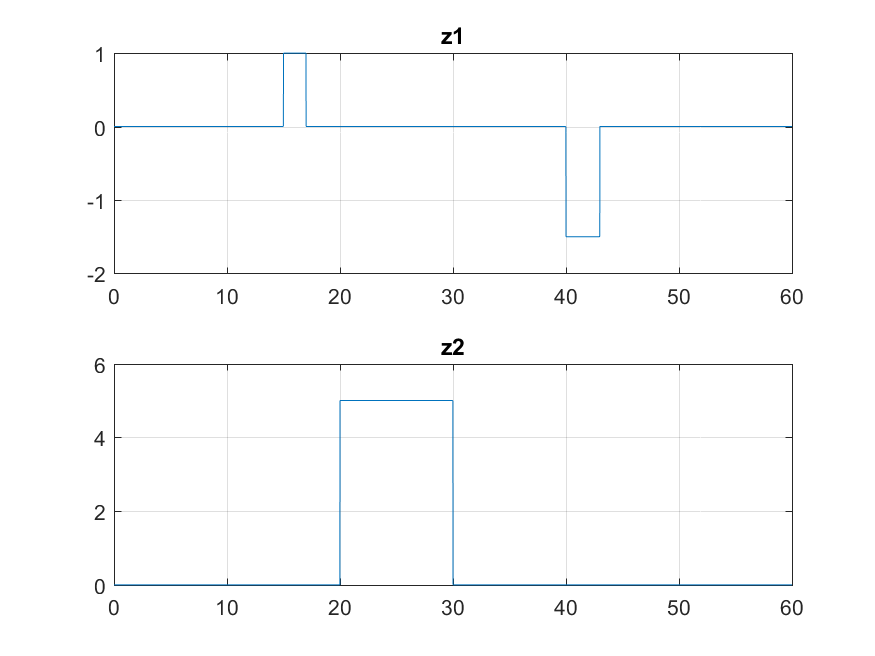
\includegraphics[scale = 0.7]{fig/Z1_New_Signal_1/fig3_1_5.png}
	\caption		
	{Zakłócenia.}
	\label{fig_zaklocenia}
\end{figure} 

Dla przedstawionych powyżej przebiegów zakłóceń przeprowadzono optymalizację a otrzymane nastawy dla poszczególnych obiektów zamieszczono w tabelach \ref{par_reg_zes1} - \ref{par_reg_zes3}. 

\begin{table}[h!]
	\centering
	\caption{Parametry regulatorów dla obiektu pierwszego rzędu.}
	\label{par_reg_zes1}
	\begin{tabular}{|c|c|c|c|c|c|c|c|}
		\hline
		\multicolumn{1}{|l|}{\begin{tabular}[c]{@{}l@{}}Parametr regulatora\textbackslash\\ Wart. zadana\end{tabular}} & $P1$ & $D1$ & $P2$ & $D2$ & $P3$ & $I3$ & $Kr$ \\ \hline
		5 & 0,1583 & 0,0000 & 0,3902 & 503,9885 & 0,0565 & 0,0393 & 1,3697 \\ \hline
		10 & 0,0875 & 0,0245 & 0,2230 & 0,3092 & 0,0454 & 0,0000 & 0,5617 \\ \hline
		20 & 0,1037 & 45,9950 & 0,4478 & 310,6393 & 0,0336 & 0,0000 & 0,5367 \\ \hline
		50 & 0,0800 & 12,6157 & 0,0000 & 4,8505 & 0,0326 & 0,0164 & 0,5671 \\ \hline
		70 & 0,0571 & 3,3536 & 0,0000 & 213,3236 & 0,0496 & 0,0331 & 0,5549 \\ \hline
	\end{tabular}
\end{table}

\begin{table}[h!]
	\centering
	\caption{Parametry regulatorów dla obiektu drugiego rzędu.}
	\label{par_reg_zes2}
	\begin{tabular}{|c|c|c|c|c|c|c|c|}
		\hline
		\multicolumn{1}{|l|}{\begin{tabular}[c]{@{}l@{}}Parametr regulatora\textbackslash\\ Wart. zadana\end{tabular}} & $P1$ & $D1$ & $P2$ & $D2$ & $P3$ & $I3$ & $Kr$ \\ \hline
		5 & 0,1036 & 0,3042 & 0,5315 & 73,9744 & 0,0442 & 0,0000 & 0,5367 \\ \hline
		10 & 0,1037 & 0,7795 & 0,5391 & 1,5989 & 0,0353 & 0,0000 & 0,5367 \\ \hline
		20 & 0,1031 & 17,033 & 0,5250 & 0,2906 & 0,0238 & 0,0000 & 0,5390 \\ \hline
		50 & 0,0800 & 0,1205 & 0,3564 & 37,7697 & 0,0509 & 0,0112 & 0,5420 \\ \hline
		70 & 0,0571 & 728,1221 & 0,2330 & 18,4368 & 0,0475 & 0,0222 & 0,5378 \\ \hline
	\end{tabular}
\end{table}

\begin{table}[h!]
	\centering
	\caption{Parametry regulatorów dla obiektu trzeciego rzędu.}
	\label{par_reg_zes3}
	\begin{tabular}{|c|c|c|c|c|c|c|c|}
		\hline
		\multicolumn{1}{|l|}{\begin{tabular}[c]{@{}l@{}}Parametr regulatora\textbackslash\\ Wart. zadana\end{tabular}} & $P1$ & $D1$ & $P2$ & $D2$ & $P3$ & $I3$ & $Kr$ \\ \hline
		5 & 0,1800 & 0,1319 & 1106,0058 & 0,4266 & 0,0143 & 0,0000 & 1,2768 \\ \hline
		10 & 0,1017 & 0,9193 & 0,4593 & 0,1072 & 0,0345 & 0,0000 & 0,5416 \\ \hline
		20 & 0,1026 & 3,2520 & 0,4596 & 123,9292 & 0,0283 & 0,0000 & 0,5438 \\ \hline
		50 & 0,0800 & 7164,0578 & 0,3120 & 6756,3846 & 0,0303 & 0,0084 & 0,5445 \\ \hline
		70 & 0,0571 & 29629,2945 & 0,1710 & 400,4956 & 0,0414 & 0,0153 & 0,5448 \\ \hline
	\end{tabular}
\end{table}

W tabeli \ref{wsk_jakosci_tab} przedstawiono wartości wskaźnika jakości dla wszystkich przeprowadzonych symulacji.

\begin{table}[h!]
	\centering
	\caption{Wartości wska\'znika jakości dla różnych wartości zadanych i różnych zestawów parametrów opisujących system.}
	\label{wsk_jakosci_tab}
	\begin{tabular}{|c|c|c|c|}
		\hline
		\multicolumn{1}{|l|}{\begin{tabular}[c]{@{}l@{}}Nr zestawu\textbackslash\\ Wart. zadana\end{tabular}} & 1 & 2 & 3 \\ \hline
		5 & 33,0087 & 43,1130 & 54,9063 \\ \hline
		10 & 38,7111 & 52,7556 & 70,6049 \\ \hline
		20 & 64,0122 & 71,5313 & 100,7350 \\ \hline
		50 & 94,3375 & 158,9382 & 195,2509 \\ \hline
		70 & 131,8947 & 198,0144 & 272,9748 \\ \hline
	\end{tabular}
\end{table}

Na rysunkach \ref{wykres_1} - \ref{wykres_4} przedstawiono przykładowe przebiegi zawierające odpowiedzi obiektów dla różnych wartości zadanych.

\begin{figure}[]
	\centering
	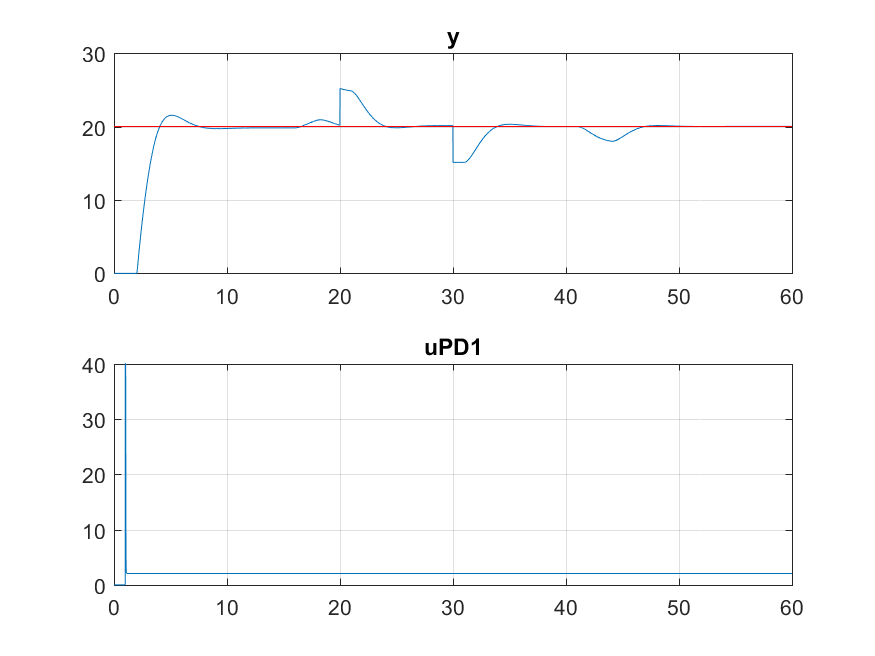
\includegraphics[scale = 0.7]{fig/Z1_New_Signal_1/fig1_2_20.png}
	\caption		
	{Odpowiedź obiektu drugiego rzędu, r = 20}
	\label{wykres_1}
\end{figure} 

\begin{figure}[]
	\centering
	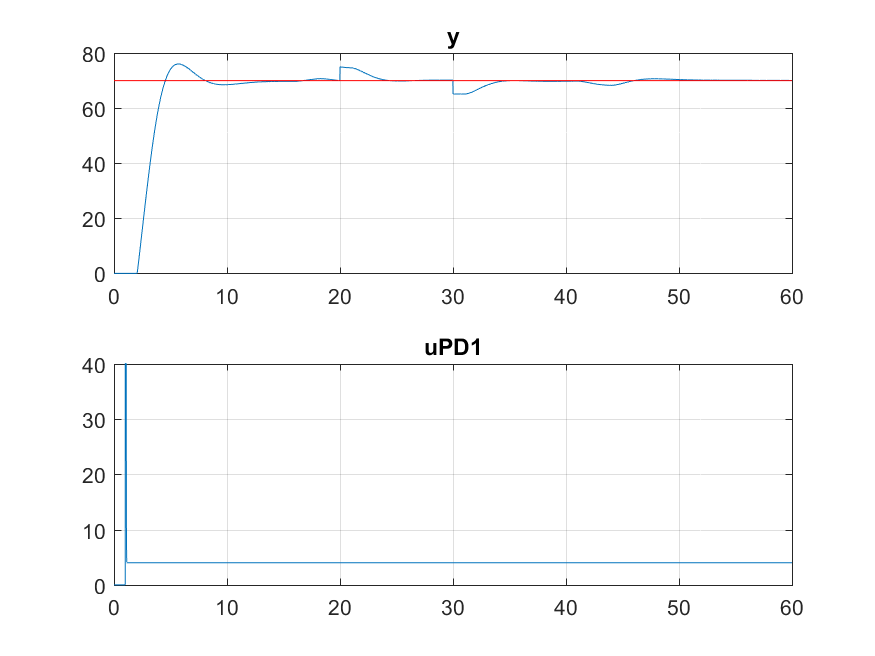
\includegraphics[scale = 0.7]{fig/Z1_New_Signal_1/fig1_2_70.png}
	\caption		
	{Odpowiedź obiektu drugiego rzędu, r = 70}
	\label{wykres_2}
\end{figure} 

\begin{figure}[]
	\centering
	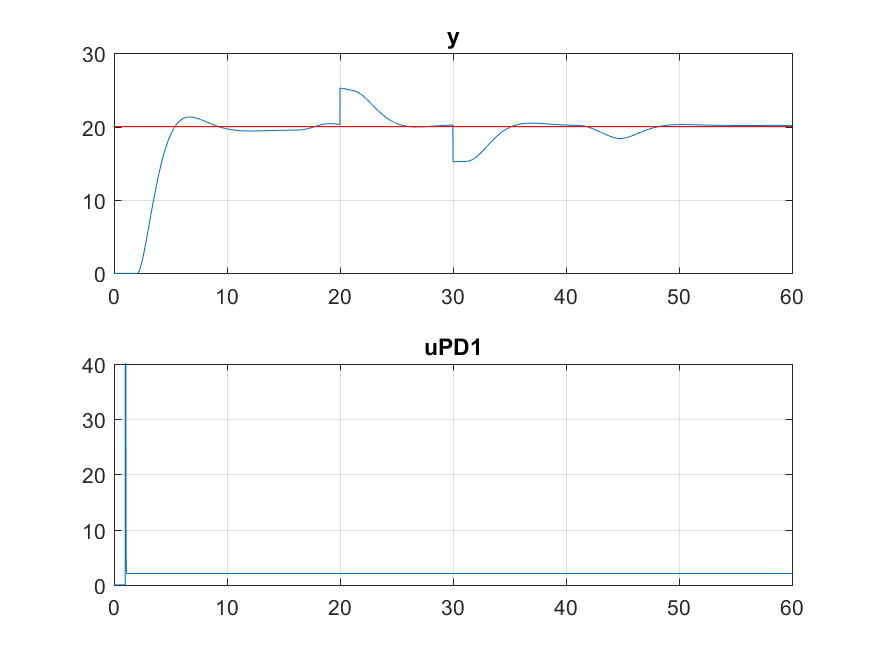
\includegraphics[scale = 0.7]{fig/Z1_New_Signal_1/fig1_3_20.png}
	\caption		
	{Odpowiedź obiektu trzeciego rzędu, r = 20}
	\label{wykres_3}
\end{figure} 

\begin{figure}[]
	\centering
	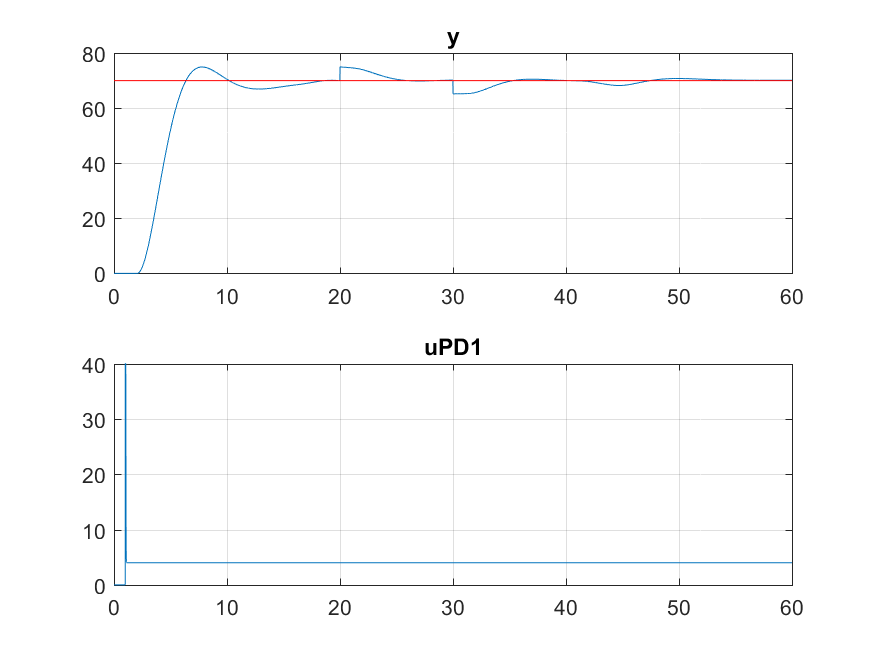
\includegraphics[scale = 0.7]{fig/Z1_New_Signal_1/fig1_3_70.png}
	\caption		
	{Odpowiedź obiektu trzeciego rzędu, r = 70}
	\label{wykres_4}
\end{figure} 